\section{State-of-the-art Text-To-SQL Methods}

\begin{figure}[htb]
  \centering
  \includegraphics[width=1\textwidth]{pics/Timeline.png}
  \caption{\small Text-to-SQL over time}
  \label{fig:timeline}
\end{figure}

This section will discuss existing cross-domain state-of-the-art (SOTA), text-to-SQL models, beginning with a broad overview and moving on to individual modules. This will provide a clear picture of the progress made in text-to-SQL research. Experiments have shown that pre-trained embeddings improve models because they construct better schema linking and a more accurate SQL structure.

An efficient text-to-SQL solution requires state-of-the-art natural language processing techniques.
As a result of the neural network's capacity to take only numerical inputs and not plain text, word embedding has been used to represent numerical words.
Aside from that, in the past few years, language models have evolved to become increasingly popular as a solution for increasing performance in natural language processing tasks.
Believing that words have numerical representations that differ from others, word embeddings aim to map each word to a multidimensional vector, incorporating valuable details about the word. In addition to the brute-force creation of one-hot embeddings, researchers have developed highly efficient methods for creating representations that convey a word's meaning and relationships with other words. In most, if not all, Text-to-SQL systems, word embedding techniques such as Word2Vec\cite{DBLP:journals/corr/Rong14}, and WordPiece embeddings\cite{DBLP:journals/corr/WuSCLNMKCGMKSJL16} are used.

Recently Language models have been shown to excel at NL tasks as a new type of pre-trained neural network. It is essential to note that language models are not a substitute for word embeddings since they are neural networks and need a way to transform words into vectors.
Relying on the specific problem they want to solve, researchers can adapt the pre-trained model's inputs and outputs and train it for an additional number of epochs on their dataset. Thus, we can achieve state-of-the-art performance without complex architectures \cite{DBLP:journals/corr/abs-1810-04805}. Recent neural network architectures, like the Transformer\cite{https://doi.org/10.48550/arxiv.1706.03762}, have been used to achieve such performance by these models, which excel at handling NL and sequences of NL that are characterized by connections between words. Several language models have been used to handle the text-to-SQL task, including BERT \cite{DBLP:journals/corr/abs-1810-04805}. BERT is a pre-trained language model that has been shown to achieve state-of-the-art performance in various NLP tasks. BERT is a Transformer-based model that utilizes a bidirectional encoder to understand the representation of a word based on the context in which it appears. BERT has been used in several text-to-SQL models, such as BRIDGE \cite{lin_bridging_2020} and RAT-SQL \cite{wang_rat_sql_2021}.



% % add image
% \begin{sidewaysfigure}
%     \centering
%     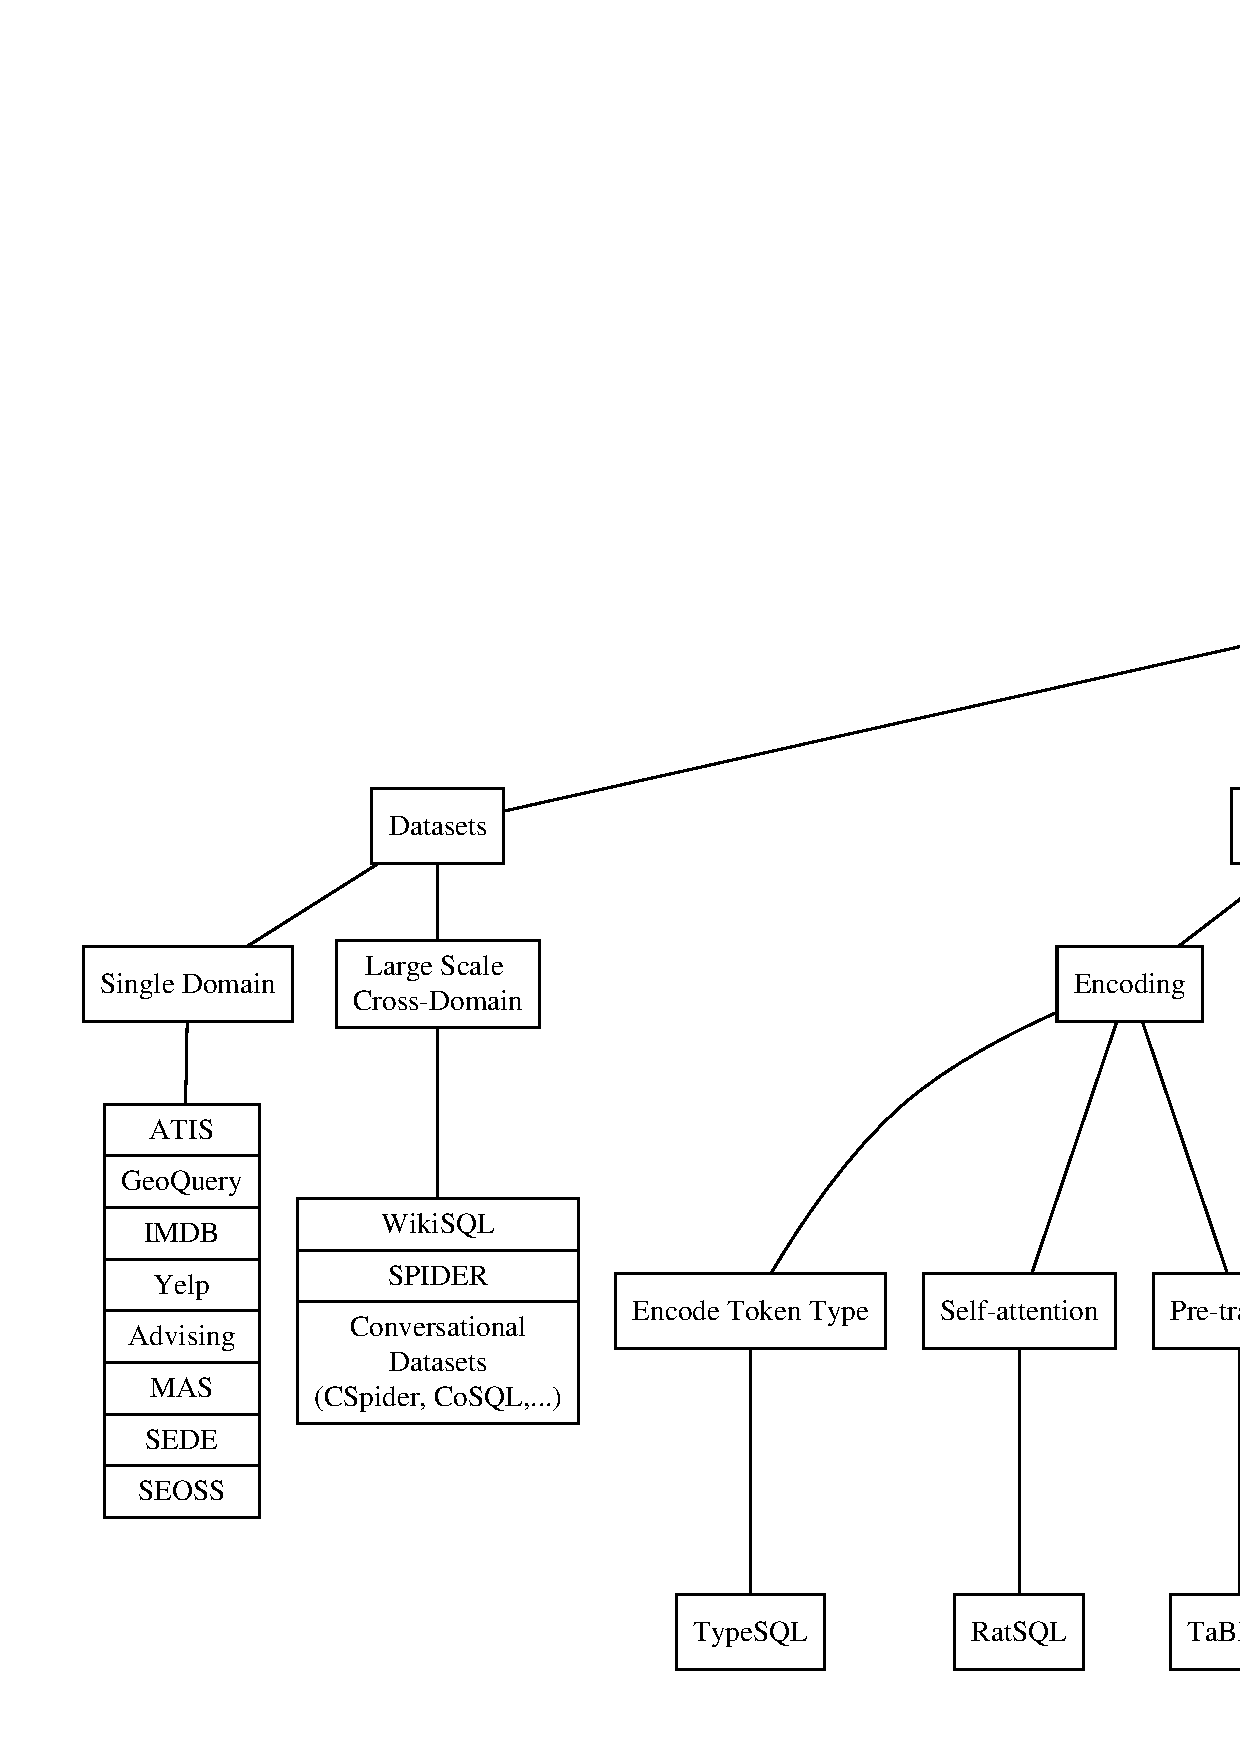
\includegraphics[width=1\linewidth]{pics/mindmap/mind}
%     \caption{Text-to-SQL state-of-the-art Topology}
%     \label{fig:mindmap}
% \end{sidewaysfigure}

\begin{figure}
    \centering
    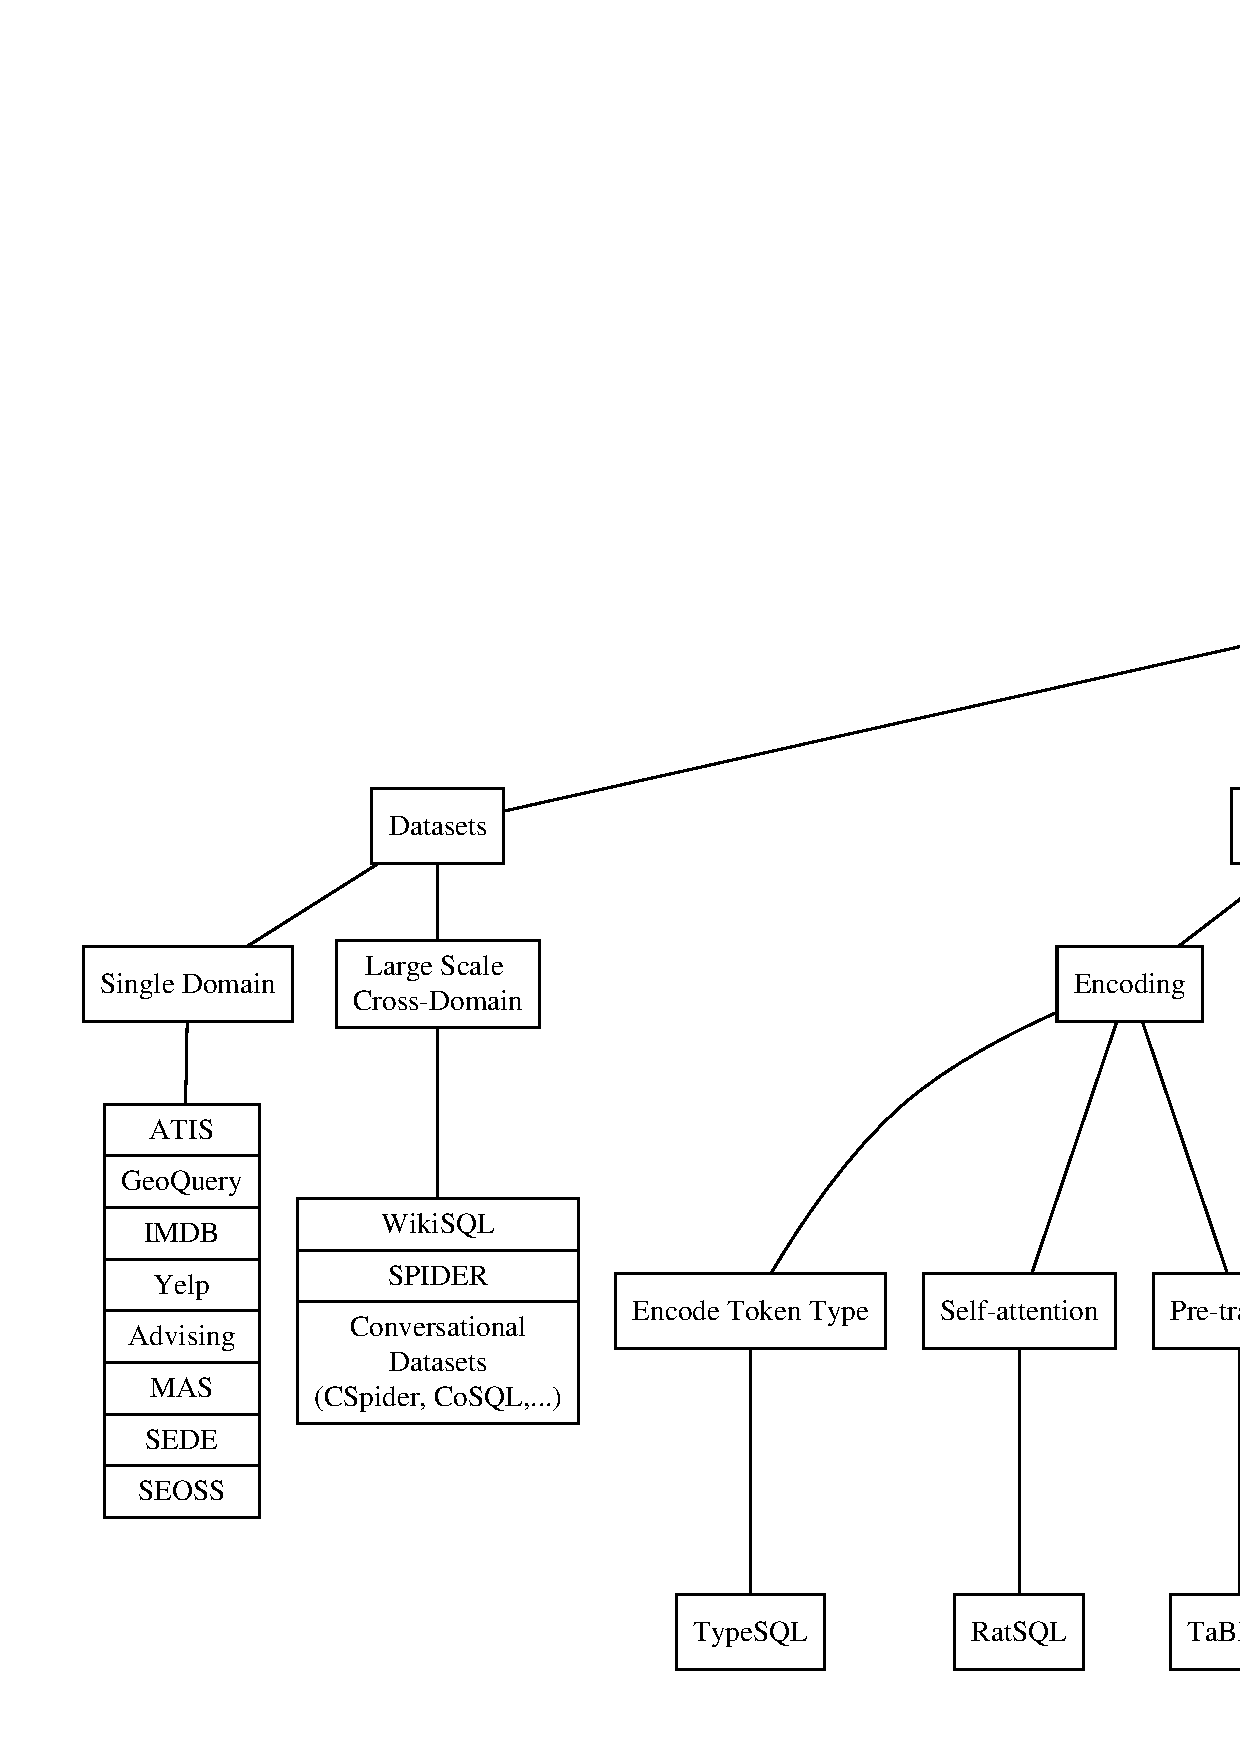
\includegraphics[width=1\linewidth]{pics/mindmap/mind}
    \caption{Text-to-SQL state-of-the-art Topology}
    \label{fig:mindmap}
\end{figure}
\clearpage
\subsection{Encoders}
\label{sec:encoders}

Several approaches have been explored to address the challenges of representing the meaning of questions, capturing the structure of database schemas, and establishing connections between database content and questions in the text-to-SQL domain. These methods play a crucial role in facilitating the understanding of the complex relationships between natural language questions and their corresponding SQL queries.

One of the main challenges in text-to-SQL research is effectively representing the meaning of questions. Various encoding methods have been used to capture the semantics of natural language questions, ranging from traditional word embeddings like Word2Vec and GloVe to more advanced contextualized representations like BERT and its variants. These encoding techniques aim to produce meaningful vector representations of questions that models can use to understand and generate accurate SQL queries.

Another important aspect is representing database schemas, which serve as blueprints for organizing and structuring databases. Researchers have used various strategies to encapsulate database schema information, such as graph-based, tree-structured, and sequence-based encodings. These approaches enable text-to-SQL models to understand the hierarchical relationships and dependencies among various database elements. This allows for more accurate and efficient query generation.

Linking database content to questions is a vital task for text-to-SQL systems. It involves the identification and mapping of relevant entities and attributes from the question to the database schema. To achieve this, various methods have been employed, including attention mechanisms, entity-linking techniques, and schema-agnostic encodings. These approaches help models identify relevant portions of the database schema and generate SQL queries that accurately reflect the intended meaning of the natural language questions.

Encoding methods and encoders play a crucial role in addressing the challenges of representing question semantics, encapsulating database schema structures, and linking database content to questions in the text-to-SQL domain. The exploration of diverse encoding techniques has led to significant advancements in the development of more accurate and efficient text-to-SQL models, furthering the field's understanding of the complex relationships between natural language questions and SQL queries.

\begin{table}
    \centering
    \newcolumntype{g}{>{\columncolor{Gray}}c}
    \begin{tabular}{|c|c|c|c|}
        \hline
        \rowcolor{Gray}
        \textbf{Methods}                & \textbf{Adopted by} & \textbf{Applied datasets} & \textbf{Addressed challenges}                                                                              \\
        \hline

        Encode token type               & TypeSQL             & WikiSQL                   & Representing question meaning                                                                              \\
        \hline
        \multirow{8}{*}{Graph-based}    & GNN                 & Spider                    & \multirow{8}{*}{\parbox{5cm}{Representing question and DB schemas in a structured way and Schema linking}} \\
                                        & Global-GCN          & Spider                    &                                                                                                            \\
                                        & IGSQL               & Sparc, CoSQL              &                                                                                                            \\
                                        & RAT-SQL             & Spider                    &                                                                                                            \\
                                        & LEGSQL              & Spider                    &                                                                                                            \\
                                        & SADGA               & Spider                    &                                                                                                            \\
                                        & ShawdowGNN          & Spider                    &                                                                                                            \\
                                        & S2SQL               & Spider                    &                                                                                                            \\
        \hline
        \multirow{5}{*}{Self-attention} & X-SQL               & WikiSQL                   & \multirow{5}{*}{\parbox{5cm}{Representing question and DB schemas in a structured way and Schema linking}} \\
                                        & SQLova              & WikiSQL                   &                                                                                                            \\
                                        & RAT-SQL             & Spider                    &                                                                                                            \\
                                        & DuoRAT              & Spider                    &                                                                                                            \\
                                        & UnifiedSKG          & WikiSQL, Spider           &                                                                                                            \\
        \hline
        \multirow{4}{*}{Adapt PLM}      & X-SQL               & WikiSQL                   & \multirow{4}{*}{\parbox{5cm}{Leveraging external data to represent question and DB schemas}}               \\
                                        & SQLova              & WikiSQL                   &                                                                                                            \\
                                        & Content Enhanced    & WikiSQL                   &                                                                                                            \\
                                        & HydraNet            & WikiSQL                   &                                                                                                            \\
        \hline
        \multirow{3}{*}{Pre-training}   & TaBERT              & Spider                    & \multirow{3}{*}{\parbox{5cm}{Leveraging external data to represent question and DB schemas}}               \\
                                        & GraPPA              & Spider                    &                                                                                                            \\
                                        & GAP                 & Spider                    &                                                                                                            \\
        \hline
    \end{tabular}
    \caption{Methods used for encoding in text-to-SQL.}
    \label{tab:methods}
\end{table}

\subsubsection{Encode Token Types}

\subsubsection{Graph-based Methods}

\subsubsection{Self-attention}

\subsubsection{Adapt PLM} %Pre-trained Language Models

\subsubsection{Pre-training}

\subsubsection{Ranking-enhanced Encoder}


\clearpage
\section{Decoders}

\begin{table}
    \centering
    \begin{tabular}{|c|c|c|c|}
        \hline
        \rowcolor{Gray}
        \textbf{Methods}                                           & \textbf{Adopted by} & \textbf{Applied datasets} & \textbf{Addressed challenges}                                                            \\
        \hline
        \multirow{3}{*}{Tree-based}                                & Seq2Tree            & -                         & \multirow{3}{*}{Hierarchical decoding}                                                   \\
                                                                   & Seq2AST             & -                         &                                                                                          \\
                                                                   & SyntaxSQLNet        & Spider                    &                                                                                          \\
        \hline
        \multirow{4}{*}{Sketch-based}                              & SQLNet              & WikiSQL                   & \multirow{4}{*}{Hierarchical decoding}                                                   \\
                                                                   &                     & WikiSQL                   &                                                                                          \\
                                                                   & IRNet               & Spider                    &                                                                                          \\
                                                                   & RYANSQL             & Spider                    &                                                                                          \\
        \hline
        Bottom-up                                                  & SmBop               & Spider                    & Hierarchical decoding                                                                    \\
        \hline
        \multirow{2}{*}{Self-Attention}                            & Seq2Tree            & -                         & \multirow{2}{*}{ Synthesizing information}                                               \\
                                                                   & Seq2SQL             & WikiSQL                   &                                                                                          \\
        \hline
        Bi-attention                                               & SmBop               & Spider                    & Synthesizing information                                                                 \\
        \hline
        Structured attention                                       & SmBop               & Spider                    & Synthesizing information                                                                 \\
        \hline
        \parbox{3cm}{Relation-aware Self-attention}                & SmBop               & Spider                    & Synthesizing information                                                                 \\
        \hline
        \multirow{4}{*}{Copy Mechanism}                            & Seq2AST             & -                         & \multirow{4}{*}{ Synthesizing information}                                               \\
                                                                   & Seq2SQL             & WikiSQL                   &                                                                                          \\
                                                                   &                     & WikiSQL                   &                                                                                          \\
                                                                   & SeqGenSQL           & WikiSQL                   &                                                                                          \\
        \hline
        \multirow{6}{*}{\parbox{3cm}{Intermediate Representation}} & IncSQL              & WikiSQL                   & \multirow{6}{*}{{\parbox{5cm}{Bridging the gap between natural language and SQL query}}} \\
                                                                   & IRNet               & WikiSQL                   &                                                                                          \\
                                                                   & ?                   & Spider                    &                                                                                          \\
                                                                   & ?                   & Spider                    &                                                                                          \\  & ?                   & GeoQuery, ATIS
                                                                   &                                                                                                                                            \\  & ?                   & Spider                    &                                                        \\
        \hline
        \multirow{2}{*}{Constrained decoding}                      & UniSAr              & WikiSQL, Spider           & \multirow{2}{*}{Fine-grained decoding}                                                   \\
                                                                   & PICARD              & Spider, CoSQL
                                                                   &                                                                                                                                            \\
        \hline
        \multirow{2}{*}{Execution-guided}                          & SQLova              & WikiSQL                   & \multirow{2}{*}{Fine-grained decoding}                                                   \\
                                                                   & ?                   & WikiSQL
                                                                   &                                                                                                                                            \\
        \hline
        \multirow{2}{*}{Discriminative re-ranking}                 & Global-GCN          &                           & \multirow{2}{*}{SQL Ranking
        }                                                                                                                                                                                                       \\
                                                                   & ?                   & Spider
                                                                   &                                                                                                                                            \\
        \hline
        \multirow{3}{*}{Constrained decoding}                      & SQLNet              & WikiSQL                   & \multirow{3}{*}{Easier decoding
        }                                                                                                                                                                                                       \\
                                                                   & ?                   & WikiSQL
                                                                   &                                                                                                                                            \\
                                                                   & ?                   & Spider
                                                                   &                                                                                                                                            \\
        \hline
        BPE                                                        & UniSAr              & WikiSQL, Spider           & Easier decoding
        \\
        \hline
        Link gating                                                & SmBop               & Spider                    & Synthesizing information                                                                 \\
        \hline
    \end{tabular}
    \caption{Methods used for encoding in text-to-SQL.}
    \label{tab:methods}
\end{table}

\subsection{Tree-based}

\subsection{Sketch-based}

\subsection{Bottom-up}

\subsection{Attention Mechanism}

\subsection{Copy Mechanism}

\subsection{Intermediate Representations}

\subsection{Prevent Invalid Tokens}

\subsection{Skeleton-aware Decoder}

Schema linking is a component of text-to-SQL models that helps map natural language phrases to elements of a database schema.
Skeleton parsing is a component of text-to-SQL models that helps generate the structure of an SQL query based on a natural language question. It focuses on generating the pure skeleton of an SQL query (i.e., SQL keywords).
\clearpage
\subsection{Data Augmentation}
\label{sec:augmentation}

Data augmentation has proven to be an effective technique for improving the performance of text-to-SQL models, allowing them to address more complex or novel questions (Zhong et al. \cite{zhong_semantic_2020} and Wang et al. \cite{wang_rat_sql_2021}), achieve cutting-edge results with less supervised data, and enhance their adaptability to various question types (Radhakrishnan et al. \cite{DBLP:journals/corr/abs-2010-09927}).

Typical data augmentation approaches involve rephrasing questions and employing pre-established templates to boost data variety. Iyer et al. \cite{iyer-etal-2017-learning} made use of the Paraphrase Database (PPDB) (Ganitkevitch et al. \cite{ganitkevitch-etal-2013-ppdb}) to create rephrased training questions. Moreover, researchers have utilized neural models to generate natural-sounding expressions for sampled SQL queries, thus broadening the available data pool. For example, Li et al. \cite{raffel_exploring_2020} fine-tuned the pre-trained Raffel T5 model \cite{raffel_exploring_2020} on WikiSQL, using the SQL query to predict natural expressions and subsequently synthesizing SQL queries from WikiSQL tables to produce corresponding natural expressions with the refined model.

The quality of the augmented data is essential, as poor-quality data can adversely affect the performance of the model\cite{DBLP:journals/corr/abs-2009-13845}. Numerous methods have been applied to enhance the quality of augmented data. Zhong et al. \cite{zhong_semantic_2020} employed an utterance generator to create natural expressions and a semantic parser to convert these expressions into SQL queries. They filtered out insufficient data by retaining only instances where generated SQL queries matched the sampled ones. Wu et al. \cite{DBLP:journals/corr/abs-2009-13845} implemented a hierarchical SQL-to-question generation process to obtain high-quality data, breaking down SQL queries into clauses, translating each clause into a sub-question, and merging the sub-questions to form a comprehensive question.

To further diversify augmented data and encourage question variety, Guo et al. \cite{DBLP:journals/corr/abs-1905-08205} incorporated a latent variable into their SQL-to-text model. Wang et al. utilized a \ac{PCFG} to explicitly model the composition of SQL queries \cite{yang-etal-2021-pcfgs}, which facilitated the sampling of compound SQL queries. These data augmentation methods collectively contribute to the enhancement of text-to-SQL models, allowing them to more effectively handle a broader range of questions and adapt to previously unencountered data.

\subsection{Results}

% add SPIDER benchmark diagram image
\begin{figure}[h]
    \centering
    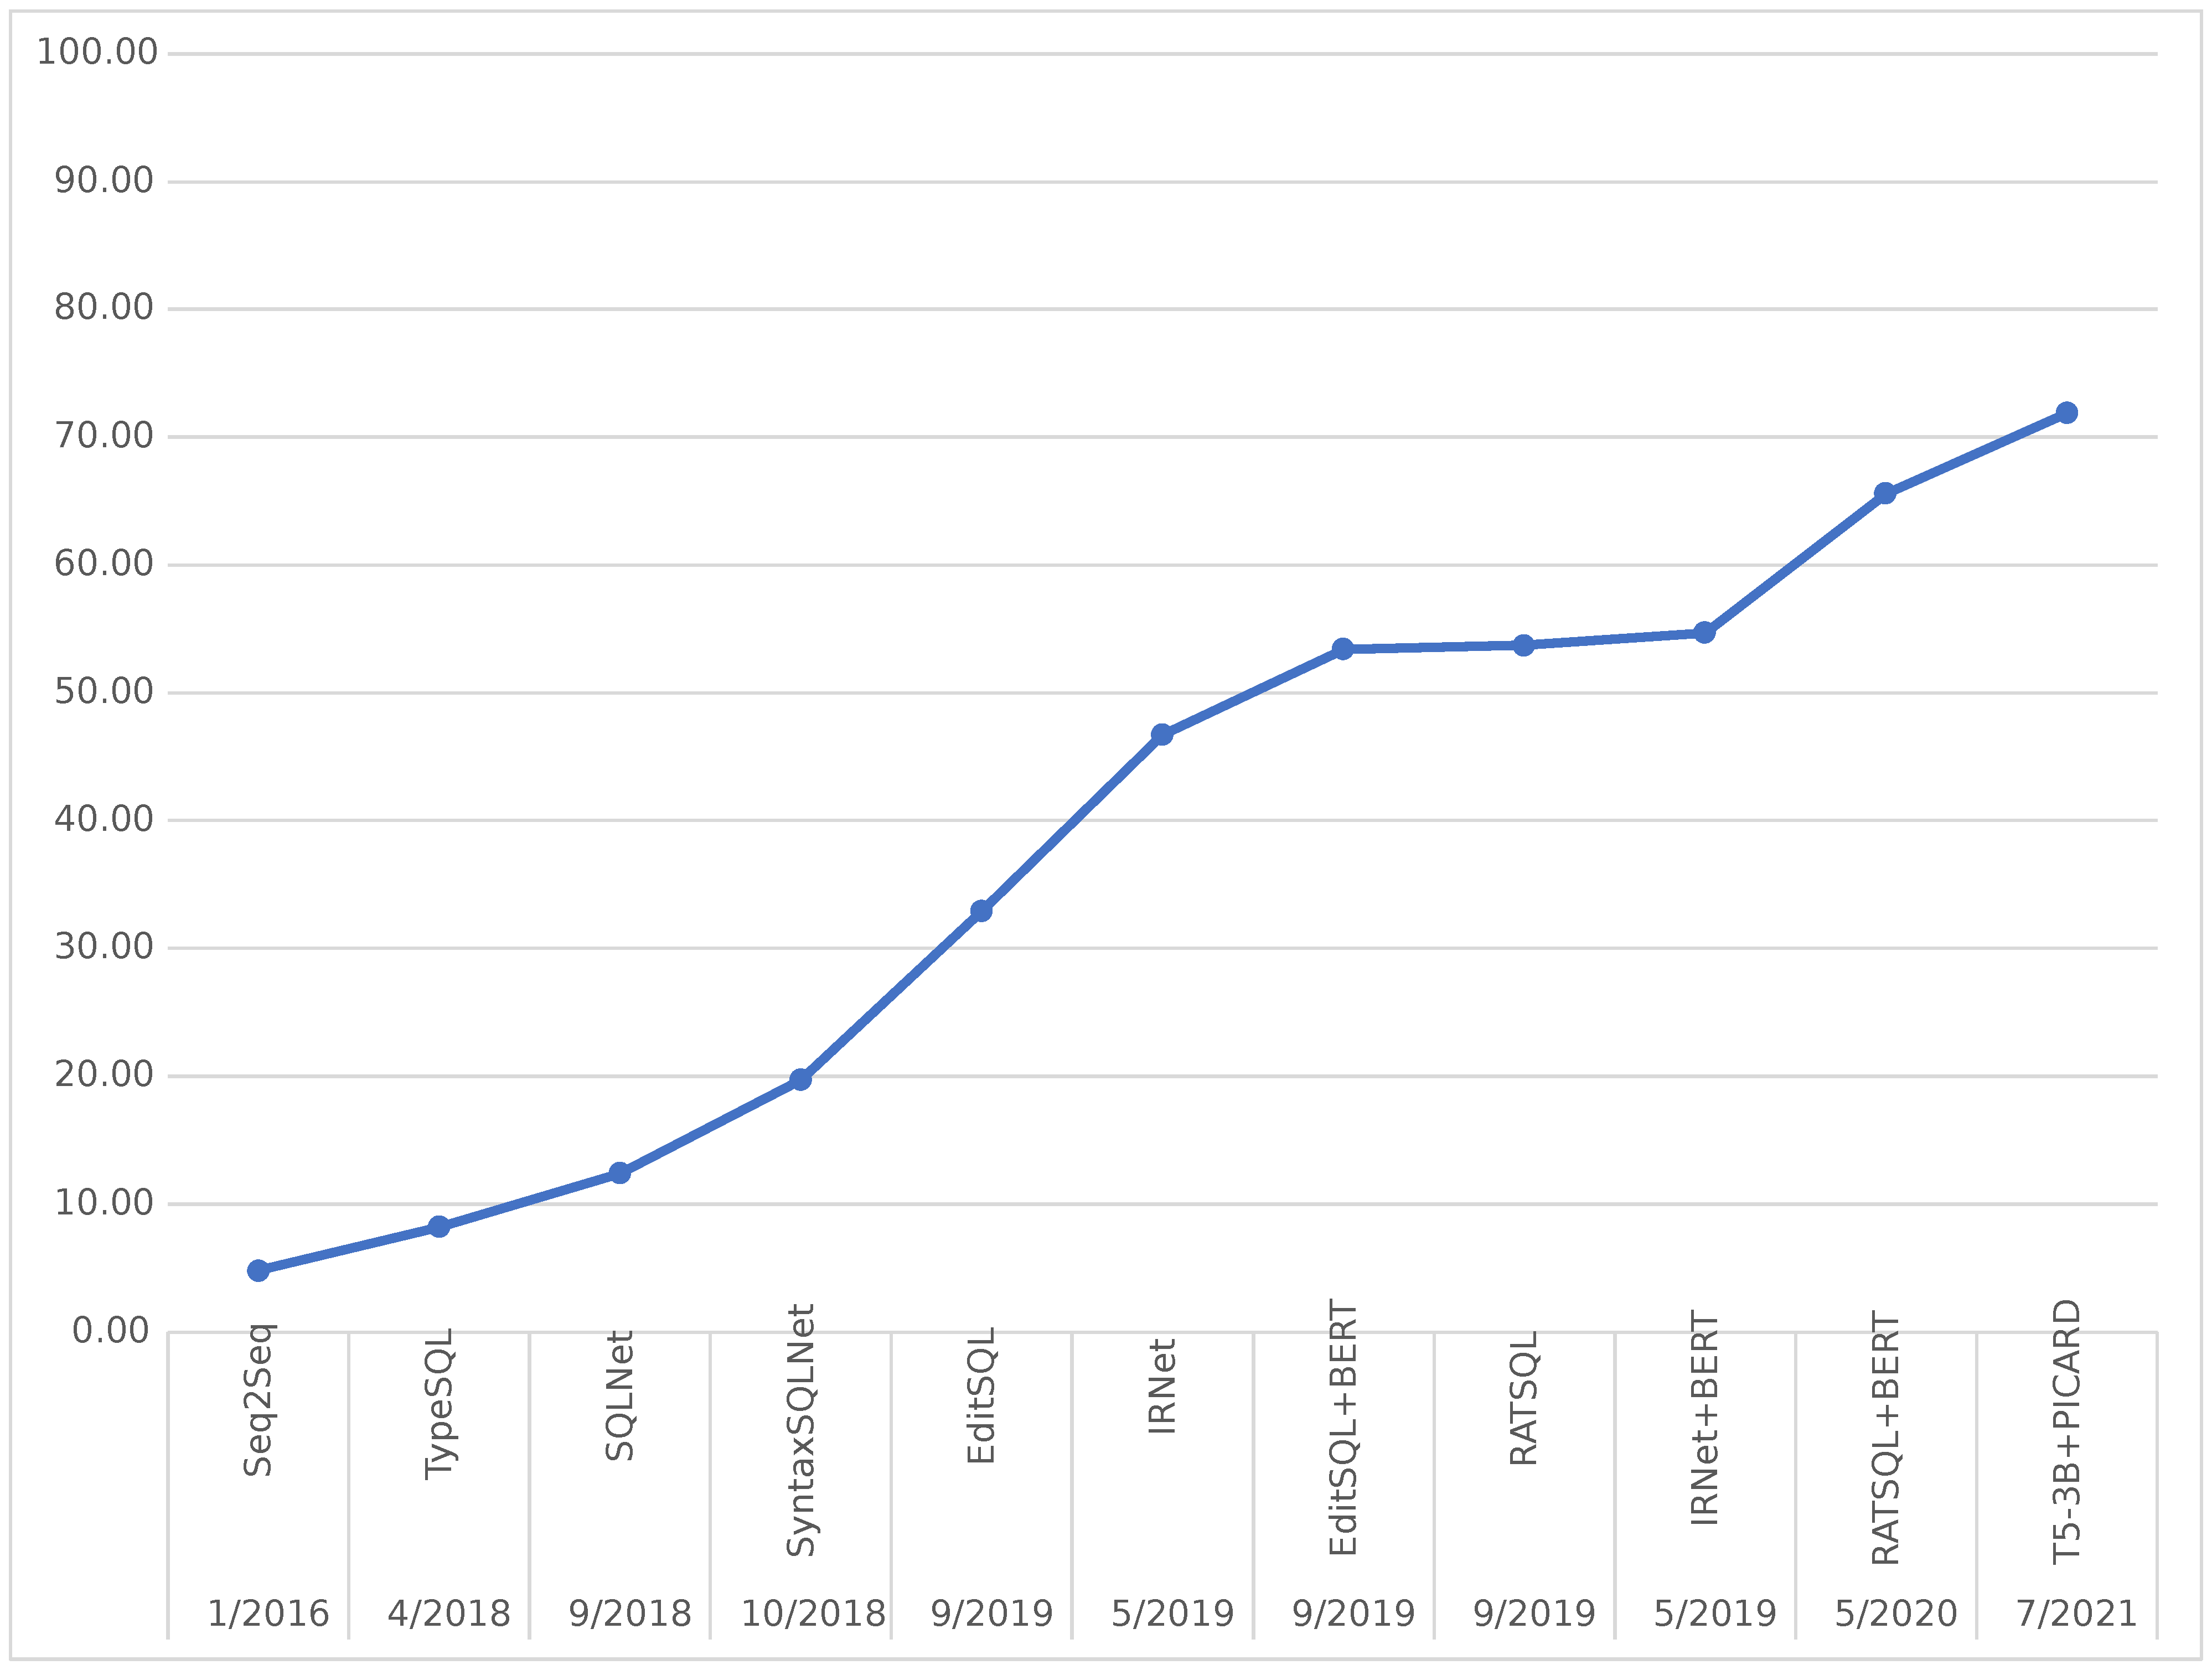
\includegraphics[width=0.99\linewidth]{pics/benchmarkeps}
    \caption{SPIDER benchmark Exact Match Results including our experiments}
    \label{fig:benchmark}
\end{figure}


Throughout this thesis, we have explored the advancements in Text-to-SQL models and their performance on the SPIDER benchmark. Our analysis revealed the significant progress made in the field, with more recent models demonstrating remarkable improvements in generating accurate SQL queries from natural language text.

The integration of powerful pre-trained language models, such as BERT, and cutting-edge architectures like T5 has played a vital role in the observed advancements. The models' ability to learn from limited labeled data, quickly adapt to new tasks or domains, and handle complex SQL queries has been substantially enhanced by employing techniques such as active learning, meta-learning, and multi-task learning.

In the following section, our experiments with ChatGPT-3.5 and ChatGPT-4.0 have showcased their superior performance, achieving scores of 81.30\% and 85.20\% on the SPIDER benchmark, respectively. These results highlight the potential of utilizing the latest huge language models for Text-to-SQL tasks, further pushing the boundaries of what is possible in this domain.

As the field of natural language processing continues to evolve, we can expect even more sophisticated models and techniques to emerge, enabling more accurate and efficient understanding and generation of SQL queries from natural language input. Future research in this area may focus on enhancing the models' ability to handle ambiguous or imprecise input, as well as exploring novel methods to improve their adaptability and generalization capabilities across diverse tasks and domains.

In the next section, we will illustrate different methods for evaluating the performance of such models.